\documentclass{beamer}
\usepackage{lmodern}

\mode<presentation>
{
  \usetheme{Boadilla}
}

\title{An Ageing Coder and His Ageing Code}
\author{Owen Campbell}
\date[DjangoCon Europe 2015]{3rd June, 2015\\DjangoCon Europe, Cardiff}

\AtBeginSection[]
{
  \begin{frame}<beamer>{Outline}
    \tableofcontents[currentsection]
  \end{frame}
}

\begin{document}

\begin{frame}
  \titlepage{}
\end{frame}

\section{Introduction}

\section{The Ageing Coder}

  \begin{frame}{Sinclair ZX81}
    \begin{columns}
      \column{0.67\textwidth}
        \begin{figure}
          \includegraphics[scale=0.25]{images/zx81}
        \end{figure}
      \column{0.33\textwidth}
        \begin{itemize}
          \item Processor: Z80 at 3.25 MHz
          \item Memory: 1 KB
          \item Storage: External Cassette Recorder
        \end{itemize}
    \end{columns}
  \end{frame}

  \begin{frame}{Ferguson 3T07}
    \begin{columns}
      \column{0.67\textwidth}
        \begin{figure}
          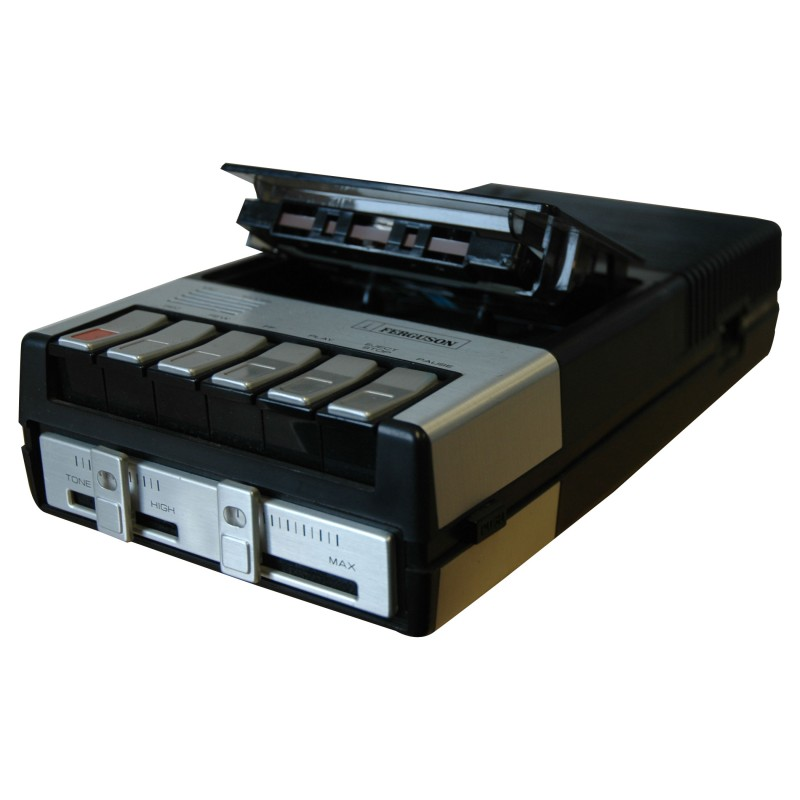
\includegraphics[scale=0.3]{images/3t07}
        \end{figure}
      \column{0.33\textwidth}
        \begin{figure}
          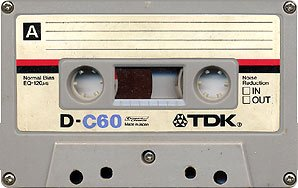
\includegraphics[scale=0.35]{images/tdkc60}
        \end{figure}
    \end{columns}
  \end{frame}

  \begin{frame}{BBC Microcomputer}
    \begin{columns}
      \column{0.67\textwidth}
        \begin{figure}
          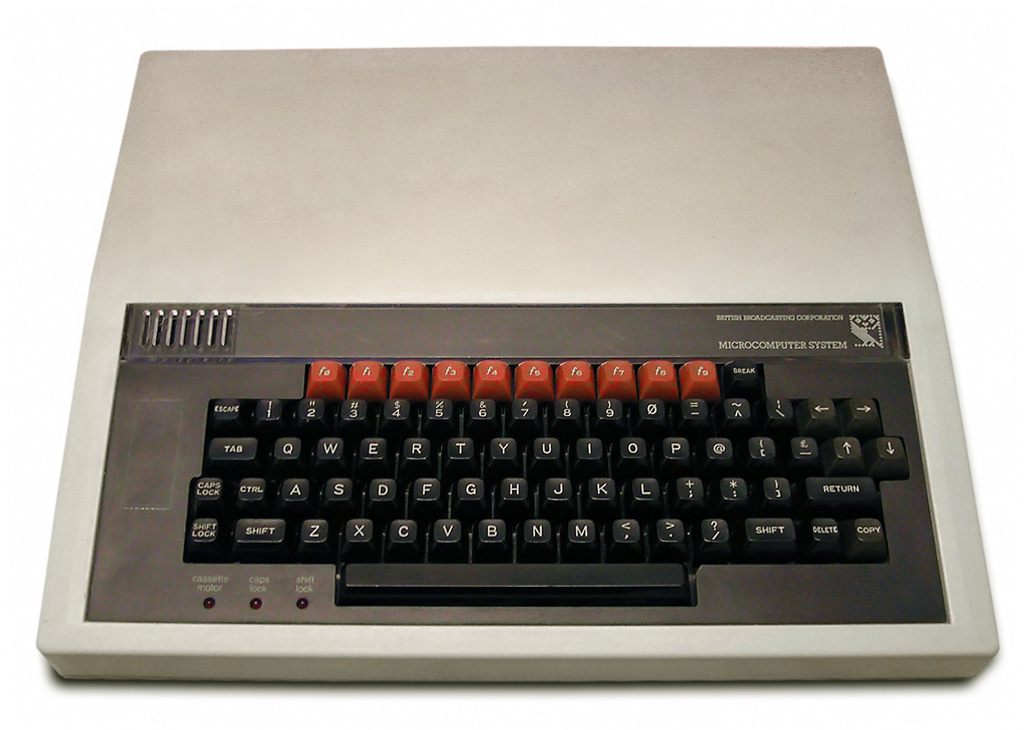
\includegraphics[scale=0.2]{images/bbc_micro}
        \end{figure}
      \column{0.33\textwidth}
    \end{columns}
  \end{frame}

  \begin{frame}{University}
    \begin{figure}
      8086 and 6800 Assembly Languages
      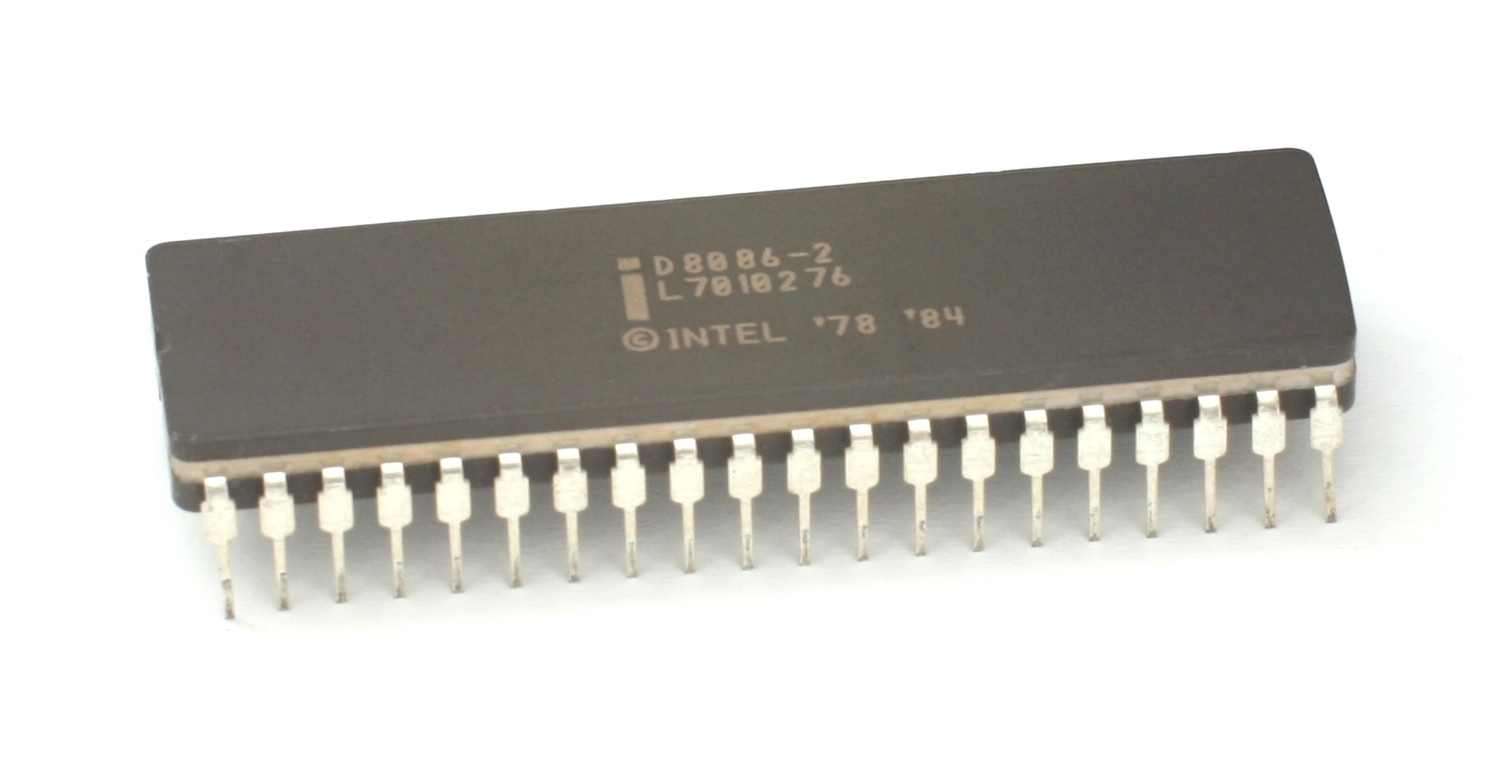
\includegraphics[scale=0.1]{images/8086}
      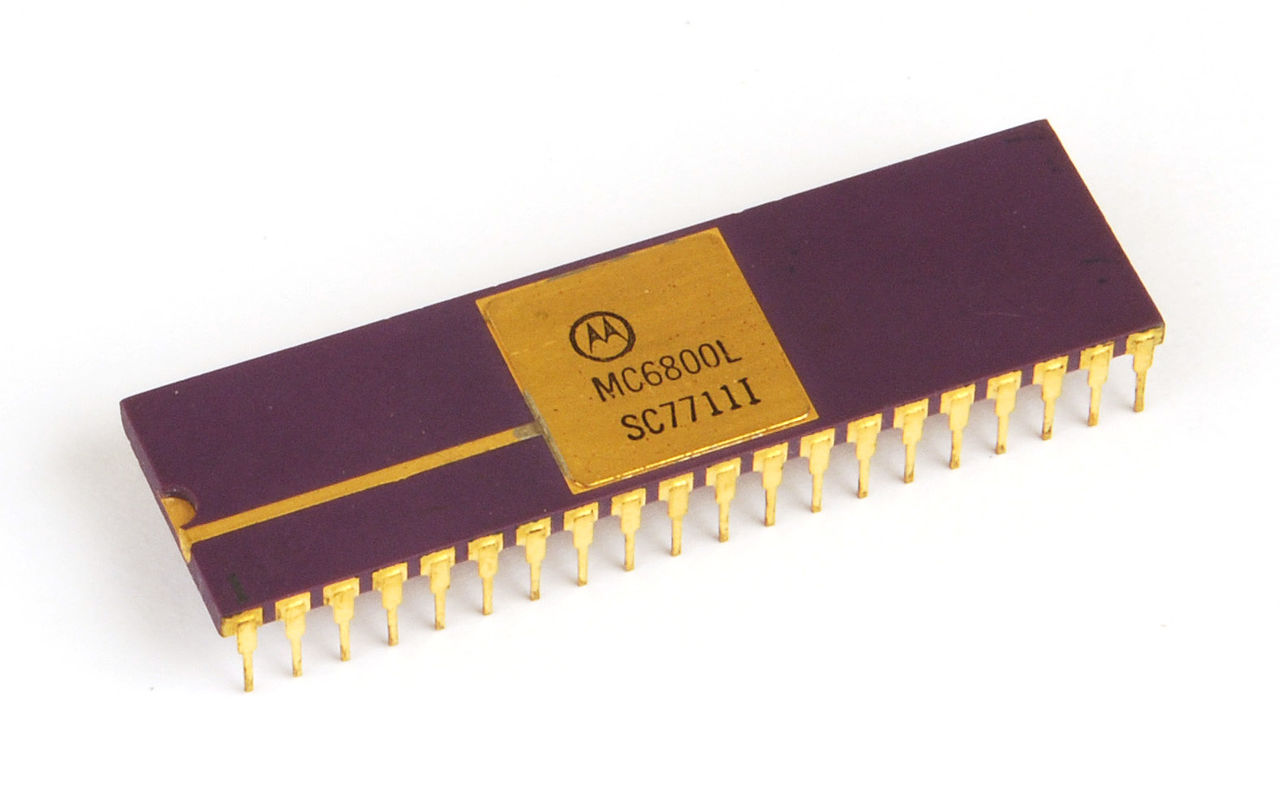
\includegraphics[scale=0.5]{images/6800}
    \end{figure}
    \begin{figure}
      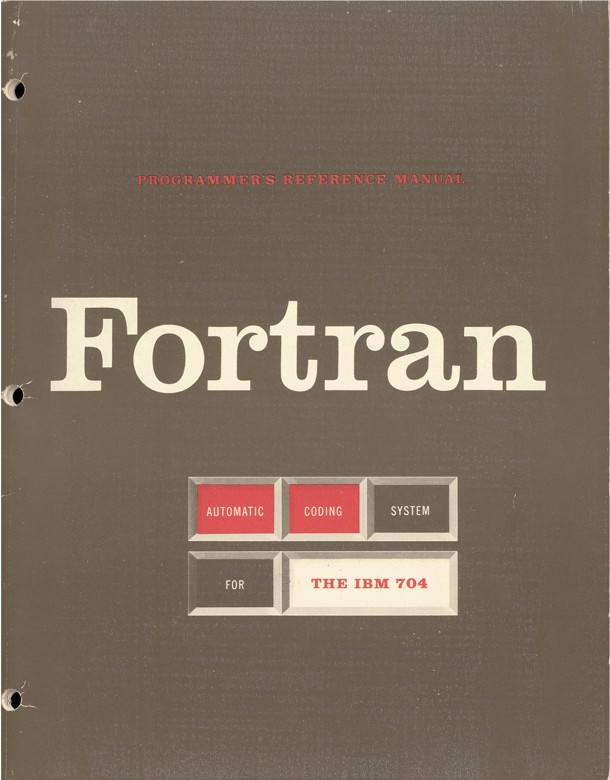
\includegraphics[scale=0.1]{images/fortran}
    \end{figure}
  \end{frame}

\section{The Ageing Code}

\section{The Way Forward}

\end{document}
